\documentclass[10pt,journal,compsoc, draftclsnofoot,onecolumn]{IEEEtran}

\usepackage{graphicx}
\usepackage{subcaption}
\usepackage{epstopdf}
\usepackage{amssymb}                                         
\usepackage{amsmath}                                         
\usepackage{amsthm}                                          

\usepackage{alltt}                                           
\usepackage{float}
\usepackage{color}
\usepackage{url}

\usepackage{balance}
\usepackage{enumitem}
\usepackage{pstricks, pst-node}

\usepackage[margin=0.75in]{geometry}
\geometry{textheight=8.5in, textwidth=6in}

\newcommand{\cred}[1]{{\color{red}#1}}
\newcommand{\cblue}[1]{{\color{blue}#1}}
\usepackage{geometry}

\usepackage{hyperref}
\usepackage{fancyvrb}
\usepackage{color}
\usepackage[latin1]{inputenc}


\makeatletter
\def\PY@reset{\let\PY@it=\relax \let\PY@bf=\relax%
    \let\PY@ul=\relax \let\PY@tc=\relax%
    \let\PY@bc=\relax \let\PY@ff=\relax}
\def\PY@tok#1{\csname PY@tok@#1\endcsname}
\def\PY@toks#1+{\ifx\relax#1\empty\else%
    \PY@tok{#1}\expandafter\PY@toks\fi}
\def\PY@do#1{\PY@bc{\PY@tc{\PY@ul{%
    \PY@it{\PY@bf{\PY@ff{#1}}}}}}}
\def\PY#1#2{\PY@reset\PY@toks#1+\relax+\PY@do{#2}}

\expandafter\def\csname PY@tok@gd\endcsname{\def\PY@tc##1{\textcolor[rgb]{0.63,0.00,0.00}{##1}}}
\expandafter\def\csname PY@tok@gu\endcsname{\let\PY@bf=\textbf\def\PY@tc##1{\textcolor[rgb]{0.50,0.00,0.50}{##1}}}
\expandafter\def\csname PY@tok@gt\endcsname{\def\PY@tc##1{\textcolor[rgb]{0.00,0.25,0.82}{##1}}}
\expandafter\def\csname PY@tok@gs\endcsname{\let\PY@bf=\textbf}
\expandafter\def\csname PY@tok@gr\endcsname{\def\PY@tc##1{\textcolor[rgb]{1.00,0.00,0.00}{##1}}}
\expandafter\def\csname PY@tok@cm\endcsname{\let\PY@it=\textit\def\PY@tc##1{\textcolor[rgb]{0.25,0.50,0.50}{##1}}}
\expandafter\def\csname PY@tok@vg\endcsname{\def\PY@tc##1{\textcolor[rgb]{0.10,0.09,0.49}{##1}}}
\expandafter\def\csname PY@tok@m\endcsname{\def\PY@tc##1{\textcolor[rgb]{0.40,0.40,0.40}{##1}}}
\expandafter\def\csname PY@tok@mh\endcsname{\def\PY@tc##1{\textcolor[rgb]{0.40,0.40,0.40}{##1}}}
\expandafter\def\csname PY@tok@go\endcsname{\def\PY@tc##1{\textcolor[rgb]{0.50,0.50,0.50}{##1}}}
\expandafter\def\csname PY@tok@ge\endcsname{\let\PY@it=\textit}
\expandafter\def\csname PY@tok@vc\endcsname{\def\PY@tc##1{\textcolor[rgb]{0.10,0.09,0.49}{##1}}}
\expandafter\def\csname PY@tok@il\endcsname{\def\PY@tc##1{\textcolor[rgb]{0.40,0.40,0.40}{##1}}}
\expandafter\def\csname PY@tok@cs\endcsname{\let\PY@it=\textit\def\PY@tc##1{\textcolor[rgb]{0.25,0.50,0.50}{##1}}}
\expandafter\def\csname PY@tok@cp\endcsname{\def\PY@tc##1{\textcolor[rgb]{0.74,0.48,0.00}{##1}}}
\expandafter\def\csname PY@tok@gi\endcsname{\def\PY@tc##1{\textcolor[rgb]{0.00,0.63,0.00}{##1}}}
\expandafter\def\csname PY@tok@gh\endcsname{\let\PY@bf=\textbf\def\PY@tc##1{\textcolor[rgb]{0.00,0.00,0.50}{##1}}}
\expandafter\def\csname PY@tok@ni\endcsname{\let\PY@bf=\textbf\def\PY@tc##1{\textcolor[rgb]{0.60,0.60,0.60}{##1}}}
\expandafter\def\csname PY@tok@nl\endcsname{\def\PY@tc##1{\textcolor[rgb]{0.63,0.63,0.00}{##1}}}
\expandafter\def\csname PY@tok@nn\endcsname{\let\PY@bf=\textbf\def\PY@tc##1{\textcolor[rgb]{0.00,0.00,1.00}{##1}}}
\expandafter\def\csname PY@tok@no\endcsname{\def\PY@tc##1{\textcolor[rgb]{0.53,0.00,0.00}{##1}}}
\expandafter\def\csname PY@tok@na\endcsname{\def\PY@tc##1{\textcolor[rgb]{0.49,0.56,0.16}{##1}}}
\expandafter\def\csname PY@tok@nb\endcsname{\def\PY@tc##1{\textcolor[rgb]{0.00,0.50,0.00}{##1}}}
\expandafter\def\csname PY@tok@nc\endcsname{\let\PY@bf=\textbf\def\PY@tc##1{\textcolor[rgb]{0.00,0.00,1.00}{##1}}}
\expandafter\def\csname PY@tok@nd\endcsname{\def\PY@tc##1{\textcolor[rgb]{0.67,0.13,1.00}{##1}}}
\expandafter\def\csname PY@tok@ne\endcsname{\let\PY@bf=\textbf\def\PY@tc##1{\textcolor[rgb]{0.82,0.25,0.23}{##1}}}
\expandafter\def\csname PY@tok@nf\endcsname{\def\PY@tc##1{\textcolor[rgb]{0.00,0.00,1.00}{##1}}}
\expandafter\def\csname PY@tok@si\endcsname{\let\PY@bf=\textbf\def\PY@tc##1{\textcolor[rgb]{0.73,0.40,0.53}{##1}}}
\expandafter\def\csname PY@tok@s2\endcsname{\def\PY@tc##1{\textcolor[rgb]{0.73,0.13,0.13}{##1}}}
\expandafter\def\csname PY@tok@vi\endcsname{\def\PY@tc##1{\textcolor[rgb]{0.10,0.09,0.49}{##1}}}
\expandafter\def\csname PY@tok@nt\endcsname{\let\PY@bf=\textbf\def\PY@tc##1{\textcolor[rgb]{0.00,0.50,0.00}{##1}}}
\expandafter\def\csname PY@tok@nv\endcsname{\def\PY@tc##1{\textcolor[rgb]{0.10,0.09,0.49}{##1}}}
\expandafter\def\csname PY@tok@s1\endcsname{\def\PY@tc##1{\textcolor[rgb]{0.73,0.13,0.13}{##1}}}
\expandafter\def\csname PY@tok@sh\endcsname{\def\PY@tc##1{\textcolor[rgb]{0.73,0.13,0.13}{##1}}}
\expandafter\def\csname PY@tok@sc\endcsname{\def\PY@tc##1{\textcolor[rgb]{0.73,0.13,0.13}{##1}}}
\expandafter\def\csname PY@tok@sx\endcsname{\def\PY@tc##1{\textcolor[rgb]{0.00,0.50,0.00}{##1}}}
\expandafter\def\csname PY@tok@bp\endcsname{\def\PY@tc##1{\textcolor[rgb]{0.00,0.50,0.00}{##1}}}
\expandafter\def\csname PY@tok@c1\endcsname{\let\PY@it=\textit\def\PY@tc##1{\textcolor[rgb]{0.25,0.50,0.50}{##1}}}
\expandafter\def\csname PY@tok@kc\endcsname{\let\PY@bf=\textbf\def\PY@tc##1{\textcolor[rgb]{0.00,0.50,0.00}{##1}}}
\expandafter\def\csname PY@tok@c\endcsname{\let\PY@it=\textit\def\PY@tc##1{\textcolor[rgb]{0.25,0.50,0.50}{##1}}}
\expandafter\def\csname PY@tok@mf\endcsname{\def\PY@tc##1{\textcolor[rgb]{0.40,0.40,0.40}{##1}}}
\expandafter\def\csname PY@tok@err\endcsname{\def\PY@bc##1{\setlength{\fboxsep}{0pt}\fcolorbox[rgb]{1.00,0.00,0.00}{1,1,1}{\strut ##1}}}
\expandafter\def\csname PY@tok@kd\endcsname{\let\PY@bf=\textbf\def\PY@tc##1{\textcolor[rgb]{0.00,0.50,0.00}{##1}}}
\expandafter\def\csname PY@tok@ss\endcsname{\def\PY@tc##1{\textcolor[rgb]{0.10,0.09,0.49}{##1}}}
\expandafter\def\csname PY@tok@sr\endcsname{\def\PY@tc##1{\textcolor[rgb]{0.73,0.40,0.53}{##1}}}
\expandafter\def\csname PY@tok@mo\endcsname{\def\PY@tc##1{\textcolor[rgb]{0.40,0.40,0.40}{##1}}}
\expandafter\def\csname PY@tok@kn\endcsname{\let\PY@bf=\textbf\def\PY@tc##1{\textcolor[rgb]{0.00,0.50,0.00}{##1}}}
\expandafter\def\csname PY@tok@mi\endcsname{\def\PY@tc##1{\textcolor[rgb]{0.40,0.40,0.40}{##1}}}
\expandafter\def\csname PY@tok@gp\endcsname{\let\PY@bf=\textbf\def\PY@tc##1{\textcolor[rgb]{0.00,0.00,0.50}{##1}}}
\expandafter\def\csname PY@tok@o\endcsname{\def\PY@tc##1{\textcolor[rgb]{0.40,0.40,0.40}{##1}}}
\expandafter\def\csname PY@tok@kr\endcsname{\let\PY@bf=\textbf\def\PY@tc##1{\textcolor[rgb]{0.00,0.50,0.00}{##1}}}
\expandafter\def\csname PY@tok@s\endcsname{\def\PY@tc##1{\textcolor[rgb]{0.73,0.13,0.13}{##1}}}
\expandafter\def\csname PY@tok@kp\endcsname{\def\PY@tc##1{\textcolor[rgb]{0.00,0.50,0.00}{##1}}}
\expandafter\def\csname PY@tok@w\endcsname{\def\PY@tc##1{\textcolor[rgb]{0.73,0.73,0.73}{##1}}}
\expandafter\def\csname PY@tok@kt\endcsname{\def\PY@tc##1{\textcolor[rgb]{0.69,0.00,0.25}{##1}}}
\expandafter\def\csname PY@tok@ow\endcsname{\let\PY@bf=\textbf\def\PY@tc##1{\textcolor[rgb]{0.67,0.13,1.00}{##1}}}
\expandafter\def\csname PY@tok@sb\endcsname{\def\PY@tc##1{\textcolor[rgb]{0.73,0.13,0.13}{##1}}}
\expandafter\def\csname PY@tok@k\endcsname{\let\PY@bf=\textbf\def\PY@tc##1{\textcolor[rgb]{0.00,0.50,0.00}{##1}}}
\expandafter\def\csname PY@tok@se\endcsname{\let\PY@bf=\textbf\def\PY@tc##1{\textcolor[rgb]{0.73,0.40,0.13}{##1}}}
\expandafter\def\csname PY@tok@sd\endcsname{\let\PY@it=\textit\def\PY@tc##1{\textcolor[rgb]{0.73,0.13,0.13}{##1}}}

\def\PYZbs{\char`\\}
\def\PYZus{\char`\_}
\def\PYZob{\char`\{}
\def\PYZcb{\char`\}}
\def\PYZca{\char`\^}
\def\PYZam{\char`\&}
\def\PYZlt{\char`\<}
\def\PYZgt{\char`\>}
\def\PYZsh{\char`\#}
\def\PYZpc{\char`\%}
\def\PYZdl{\char`\$}
\def\PYZti{\char`\~}
% for compatibility with earlier versions
\def\PYZat{@}
\def\PYZlb{[}
\def\PYZrb{]}
\makeatother


\begin{document}

\title{Design Document\\ 3D Object Pose Tracking for Robotics Grasping \\ CS461 Fall 2018}
\author{Connor Campbell, Chase McWhirt and Jiawei Mo}

\maketitle

\begin{abstract}
Robotic vision is an advanced topic that requires proper planning and consideration before attempting. In this project, a computer will be taught to recognize a robotic arm in an image by first narrowing down the region of the image it is likely in, then scanning the area with a neural networks. Different solutions as well as technologies used for achieving them are discussed.
\end{abstract}

\IEEEdisplaynontitleabstractindextext
\IEEEpeerreviewmaketitle

\newpage
\pagebreak
\tableofcontents
\pagebreak

\section{Introduction}
\subsection{Purpose}
The goal of this document is provide a clear path of execution to stakeholders about how this product development project will reach completion.It should ensure that the client, the instructors, and the students all understand how this project will be completed.

\subsection{Scope}
This document will describe various technologies, design choices, and a measurable progress checklist that will guide the rest of this product development project.

\subsection{Context}
This document is being written not only as a road map for our stakeholder, but also for our teachers and teachers' assistants to follow. The project must be feasible to complete to the specifications by March 22, the end of Winter term, 2019. If the project isn't completed by this time, there is only minimal flexibility available before the Oregon State Engineering Expo on May 17.

\subsection{Summary}
The end goal of this project is to create a software that will accurately identify a robotic arm in a given image. Several possible solution plans have been created with the help of the client. The client is going to take many photos (as HSV image type) of the robotic arm and supply a mathematical description of the arm's pose for each photo. Next, a straw man solution will be generated by running a k-means clustering method on all of the images, which will yield a naive method for identifying parts of the robotic arm. This will act as a base line: the other solutions will be considered successful if the prove to be better than the straw man solution. \\

\noindent
The images will be categorized based on the robotic arm's pose, with each category having a key pose, and the images assigned to a category using a nearest neighbor algorithm. The other solutions will work using those categorizations. \\

\noindent
The first possible solution is to run k-means on each of the pose groups. The other solution is to train small neural networks on each subgroup. The client suggested two hidden layers of eight nodes each for these networks. With six inputs and two outputs, it should not be too time consuming to train each neural network. 10\% of the data, will be set aside to test the effectiveness of each neural network. This check will be run against an ROC (receiver operating characteristic) curve. \\

\noindent
Finally, as a backup plan, if none of the solutions performs better than the straw man (or perhaps to run alongside the three solutions regardless) A neural network will be trained on all of the data (without pose nearest neighbor groupings) to see if it can get better results. This will also be tested with 10\% of the data against an ROC curve.



\section{Glossary}
\noindent \textbf{Caffe}: A deep learning framework developed by Berkeley AI Research (BAIR) and by community contributors. \\

\noindent \textbf{Gimp}: GNU Image Manipulation Program, an open source graphics editor, is merged with new features by various developers and GIMP team will authorize the source to avoid corruption. \\

\noindent \textbf{HSV}: Stands for Hue, Saturation and Value. It is a color model used for defining colors in computer graphics. \\

\noindent \textbf{K-means clustering}: A method of dividing a large set of data into smaller portions based on where the data points tend to cluster. \\

\noindent \textbf{Neural Network}: A type of machine learning algorithm that can be trained to solve a variety of problems. Several layers of nodes simulate the firing of neurons. \\

\noindent \textbf{OpenCV}: An open source library for computer vision field. It was initially released in 2000 and written in C/C++. It supports various operating system and has interfaces for different programming languages, including Python, C and C++. The latest version is 4.0.0. \\

\noindent \textbf{RBG}: Stands for Red, Blue and Green. A different color model. \\

\section{Stakeholders and Design Concerns}
There are three primary stakeholders vested in this project. The first is the client and sponsor, Cindy Grimm, whose primary concerns are completion of the project within particular specifications. There are also the instructors, Kevin McGrath and Kirsten Winters, and the teaching assistant assigned to this project Wesley  Alexis. Their primary concerns are upholding mandatory standards of practice and quality assurance. While in the context of the class, we should consider all stakeholders and concerns, this document will focus on the client's concerns.


\section{Design Aspects}

\subsection{Neural Network API}
Our completed project will be using neural networks. Overall, we'll be using a supervised learning approach. Caffe \cite{3:online} is a robust, flexible framework that works well for this project in many ways. It's easy to work with, works efficiently, and is tailored for many project specifications. This framework is classified as a deep learning framework. For proper implementation, three deep learning principles should be considered. Deep learning uses a cascade of multiple layers of nonlinear processing units for feature extraction and transformation. As a project specification, implementation will follow supervised learning. Finally, the neural networks will learn multiple levels of representation that correspond to different levels of abstraction; the levels form a hierarchy of concepts \cite{deep_learning}.



\subsection{Qualifying Data}
Supervised learning requires a neural network to be shown several example problems along with the desired outcome. As such, not only will we need a large data set of images (which our client will be providing for us), but the images in our data will need to be properly labeled with the desired outcome, which needs to be done by hand. Specifically, each pixel in the image will need to be labeled as either part of the arm or not part of the arm. This will require the use of image editing software that can trace objects. Our goal is to turn raw data into qualified, supervised data. \\

\noindent Gimp will be used to fulfill this need. Gimp is an open source and free software that will have the capability of qualifying the image feed \cite{4:online}. This will increase accessibility to the software. In turn, we'll be able to quickly qualify data that our neural networks can train with.


\subsection{Input Images}
\noindent
Once the sets of images of the arm are prepared, the next step is to read images into the software for training. This will require storing images and information about them in a way that the software can understand, as well as the ability to manipulate that information. \\

\noindent
In order to store and manipulate images, OpenCV will be used. OpenCV is an open source C/C++ library aimed at solving computer vision problems \cite{1:online}. OpenCV stores the pixels of an image in a matrix. Depending on the type of picture, each pixel can hold various values representing their color. Each value in the matrix can represent a variable of RGB (BGR instead of RGB in OpenCV functions) or gray scale. A pixel's color is described and manipulated through the use of a channel, which stores many values related to the pixel and automatically adjusts related values when one is changed. For instance, it can convert from BGR to HSV and vice versa, which allows for HSV to be used even if the image is based on the RGB color system. For the purposes of this project, OpenCV will convert the colors of the pixels in an image into a set of values that the software will understand.

\subsection{Mask Operation}
A method of narrowing down the general region where the arm can be found will be used to reduce the strain on the neural networks. An object in an image will generally have similarly colored pixels. The mask operation essentially looks for sudden changes in color within an image to determine approximate boundaries for different objects. After obtaining an approximate area, the neural network will be tasked with providing a more precise identification. The client suggests using the K-means algorithm for this as well.

\begin{figure}[h!]
    \centering
    \begin{subfigure}[b]{0.15\textwidth}
        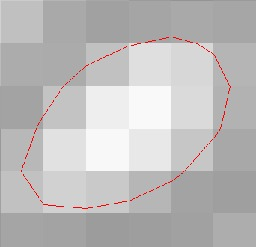
\includegraphics[width=\textwidth]{unmasked.jpg}
        \caption{Before Masking}
    \end{subfigure}
    ~ %add desired spacing between images, e. g. ~, \quad, \qquad, \hfill etc. 
      %(or a blank line to force the subfigure onto a new line)
    \begin{subfigure}[b]{0.15\textwidth}
        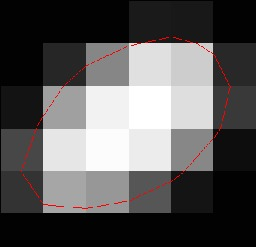
\includegraphics[width=\textwidth]{soft_masking.jpg}
        \caption{Soft Masking}
    \end{subfigure}
    ~ %add desired spacing between images, e. g. ~, \quad, \qquad, \hfill etc. 
    %(or a blank line to force the subfigure onto a new line)
    \begin{subfigure}[b]{0.15\textwidth}
        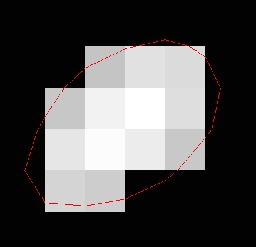
\includegraphics[width=\textwidth]{hard_masking.jpg}
        \caption{Hard Masking}
    \end{subfigure}
    \caption{An example of a masking operation}\label{fig:animals}
\end{figure}

\noindent
Figure 1 demonstrates an example use of a masking operation \cite{2:online}. In this project, the operation will be used to remove irrelevant information (ie. anything that isn't the robotic hand). 


\section{Design Rationale}
Clearly, this project is beyond our expected level of knowledge. With this in mind, it is clear that opting for tools that can be tried quickly and repeatedly is critical to a successful end product. It is possible that we'll change our planned implementation along the way and will require the reworking of fundamental steps along our path. With the tools that have been designated, sudden changes will not be catastrophic to the project.


\section{Conclusion}
 Upon project completion, the computer will be able to identify the robot arm in real time.
At least one of the methods used will beat the straw man approach of k-mean clustering without applying nearest neighbor.
Ideally, the computer will be able to identify 80-90\% of the arm in real time with false positives being more acceptable than false negatives.
However, if this arbitrary metric is not achieved, it will show that this approach will not generally
be successful and an alternate approach (being developed by another person) will be used instead.
If this method proves successful before the deadline, there are also some stretch goals for the project, such as performing similar methods with objects for the robot to pick up.
Another stretch goal is to ensure that both methods can run simultaneously in real time.


\newpage
% bibliography
\nocite{*}%if nothing is referenced it will still show up in refs
\bibliographystyle{ieeetr}
\bibliography{refs}
%end bibliography
\end{document}